\documentclass[a4paper,11pt]{article}
\usepackage[T1]{fontenc}
\usepackage[utf8]{inputenc}
\usepackage{lmodern} 
\usepackage[portuguese]{babel}
\usepackage{graphicx}			%para imagens
\usepackage{epstopdf} 			%resolve problemas eps-pdf
\usepackage{fancyhdr}			% para o cabeçalho bonito
\usepackage{caption}				%para legendas
\usepackage{subcaption}			% e sublegendas
\usepackage{placeins} 			%controlar o lugar dos floats
\pagestyle{fancy} 				% número de pag e cabeçalho
\usepackage{slashbox} 			% criando caixas maneiras
\usepackage{wrapfig} 			%texto em volta da imagem
\usepackage{txfonts} 			%fontes bonitas? acho que para o título
\usepackage[usenames]{color} 	% algo com gunplot e eps
\graphicspath{{./images/}}		% procura imagens nessa pasta



\newcommand{\HRule}{\rule{\linewidth}{0.5mm}}


%@@@@@@@@@@@@@@@@      Cabeçalho de cada página      @@@@@@@@@@@@@@@@@@@@@@

\setlength{\headheight}{15pt}%compila sem erro
	\fancyhead{}
	\fancyfoot{}
	\fancyhead[R]{Física Experimental 4}%direito superior
	\fancyhead[L]{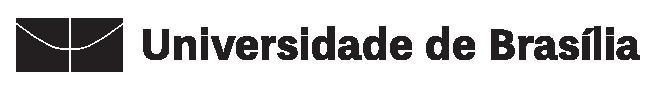
\includegraphics[height=0.25in]{logo_unb.eps}}%esquerda superior
	\fancyfoot[C]{\thepage}%baixo centro
%E: Even page, O: Odd page, L: Left field, C: Center field, R: Right field, H: Header, F: Footer
% em documentos com dois lados use LO, RO. como esse documento não tem lados essa opção é inútil


\begin{document}
\begin{titlepage}
\begin{center}

% Upper part of the page. The '~' is needed because \\
% only works if a paragraph has started.

\includegraphics[width=\textwidth]{logo_unb.pdf}~\\[1cm]

\Huge Física Experimental 4\\[0.5cm]

\huge Experimento III

% Title
\HRule \\[0.4cm]
{ \huge \bfseries  Decaimento da Intensidade Luminosa e Coeficientes de Absorção e Reflexão}\\[0.4cm]

\HRule \\[0.5cm]

{\large \today}


\vfill %%o que vier depois vai ao fim da páginda


% Author and supervisor

	\begin{center} \large
		\begin{tabular}{llr} \
		& & \\[0.05cm]		
		Professora & Nadia Maria de Liz Koche & \\
		
		Alunos:& & \\
		& Juarez A.S.F 					& 11/0032829\\
		& Sérgio Fernandes da Silva Reis & 11/0140257\\
		& Jedhai Pimentel				& 09/0007883\\	[0.05cm]	
		\end{tabular}

	
	\end{center}


\end{center}
\end{titlepage}

\tableofcontents

\newpage

%@@@@@@@@@@@@@@@@@@@@@@@@@@@@@@@@@@@@@@@@@@@@@@@@@@@@@@@@@@@
%@@@@@@@@@@@@@@@@      OBJETIVOS      @@@@@@@@@@@@@@@@@@@@@@
%@@@@@@@@@@@@@@@@@@@@@@@@@@@@@@@@@@@@@@@@@@@@@@@@@@@@@@@@@@@
\section{Objetivos}
\paragraph{} Este experimento visa observar o campo elétrico $ \vec{E} $ e o campo magnético $ \vec{B} $ presentes em uma onda eletromagnética e observar o comportamento desta diante uma grade e uma placa ambas feitas de material condutor. 

%@@@@@@@@@@@@@@@@@@@@@@@@@@@@@@@@@@@@@@@@@@@@@@@@@@@@@@@@@@@
%@@@@@@@@@@@@@@@        MATERIAIS         @@@@@@@@@@@@@@@@@@
%@@@@@@@@@@@@@@@@@@@@@@@@@@@@@@@@@@@@@@@@@@@@@@@@@@@@@@@@@@@
\section{Materiais}
\paragraph{} Este experimento fará uso de:
\begin{itemize}
\item[•] Fonte de micro-ondas
\item[•] Detetor sensível de campo elétrico
\item[•] Detetor sensível de campo magnético
\item[•] 2 Microamperímetros
\item[•] Banco ótico para suporte dos detetores
\item[•] Grade metálica
\item[•] Chapa metálica
\item[•] Régua milimetrada 
\end{itemize}
\newpage
%@@@@@@@@@@@@@@@@@@@@@@@@@@@@@@@@@@@@@@@@@@@@@@@@@@@@@@@@@@@
%@@@@@@@@@@@@@@        INTRODUCAO       @@@@@@@@@@@@@@@@@@@@
%@@@@@@@@@@@@@@@@@@@@@@@@@@@@@@@@@@@@@@@@@@@@@@@@@@@@@@@@@@@

\section{Introdução}
\paragraph{} Matematicamente, onda é qualquer forma que satisfaça a equação diferencial :
\begin{equation}
\frac{\partial ^2}{\partial t^2 }\Psi = k^2 \frac{\partial ^2}{\partial x^2 }\Psi ,\: k \in \Re
\label{eq-onda}
\end{equation}

\paragraph{} Fisicamente uma onda é um distúrbio ou oscilação que se propaga pelo espaço e pela matéria acompanhada por uma transferência de energia. O tipo de onda em estudo, a eletromagnética, é a propagação de uma perturbação em campos elétricos e/ou magnéticos. Pode ser mostrado que as equações governantes dos fenômenos elétricos e magnéticos geram uma equação de onda como mostrada em \ref{eq-onda}.

\paragraph{}O experimento requer o entendimento de duas equações:
\begin{equation}
\oint \vec{E} \cdot d\vec{s} = -\frac{d}{dt}\Phi_B
\label{eq-faraday}
\end{equation}
\begin{equation}
E_s = -\frac{\partial}{\partial s}V
\label{eq-E-V}
\end{equation}


\paragraph{}A equação \ref{eq-faraday} é conhecida como a Lei de Faraday e ela nos diz que a variação do fluxo magnético faz surgir um campo elétrico. A equação \ref{eq-E-V} nos diz que um campo elétrico faz variar a força eletromotriz em um circuito. Essas duas equações serão usadas no entendimento dos detetores de campo utilizados no experimento.

\paragraph{}Considere o detector mostrado na figura \ref{detetor-E}. A equação \ref{eq-E-V} nos diz que um campo elétrico incidente nas antenas irá gerar uma ddp no circuito e portanto uma corrente. Para que vejamos a corrente é necessário que o campo elétrico oscilante chegue no plano das antenas. Seja agora o detector na figura \ref{detetor-B}. A equação \ref{eq-faraday} nos diz que se fizemos variar o fluxo magnético no interior deste circuito teremos um campo elétrico.Pela equação \ref{eq-E-V} temos o surgimento de uma ddp no circuito e portanto uma corrente. Para isso é preciso que a onda passe por dentro da espira formada pelo circuito, ou seja, o plano do detector deve estar perpendicular à direção de propagação da onda.\footnote{Os diodos retificadores são usados nos detetores apenas para transformar o sinal AC produzido pelos campos em sinal DC e facilitar as observações}

\FloatBarrier
\begin{figure}[!htp]
			\centering
			\begin{subfigure}[b]{0.3\textwidth}
					\centering					
					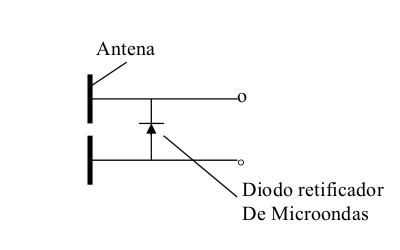
\includegraphics[scale=0.6]{detetor-E.jpg}
					\caption{Elétrico}
					\label{detetor-E}
			\end{subfigure}
			\qquad
			\begin{subfigure}[b]{0.3\textwidth}
					\centering
					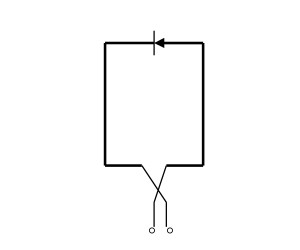
\includegraphics[scale=0.6]{detetor-B.jpg}
					\caption{Magnético}
					\label{detetor-B}
			\end{subfigure}
			
	\caption{Detetores de campo}
	\end{figure}
\FloatBarrier

	\paragraph{}  Notamos que em ambos os detectores criados a corrente que surgirá no circuito deve ser proporcional ao campo medido. Temos então uma ferramenta para observar os campos $ \vec{E} $ e $ \vec{B} $. 
	
	\paragraph{} Podemos agora observar a polarização da onda EM. Um polarizador é um objeto que permite a passagem apenas de ondas com uma certa orientação. A princípio os campos campos $ \vec{E} $ e $ \vec{B} $ podem estar orientados em qualquer plano \footnote{O que se sabe é que os campos $\vec{E} $ e $ \vec{B}$ são perpendiculares em relação à direção de propagação e entre si}. Colocando um polarizador em várias direções e observando o comportamento da onda em estudo podemos determinar se existe um plano que a oriente.
	
	\paragraph{} O outro efeito estudado será a formação de uma onda EM estacionária. Uma onda estacionária é aquela na qual a forma da onda não se propaga em um sentido, as posições de máximos e mínimos não variam com o tempo. A forma será atingida ao fazermos interferir a onda da fonte com a onda refletida de uma chapa metálica. Quando isso acontece a onda EM formada possui a forma:
	\begin{equation}
	\begin{array}{c}
		E(x,t) = -2 E_{max}\sin(\frac{2\pi}{\lambda}x)\cos(wt) \\
		B(x,t) = 2 B_{max}\cos(\frac{2\pi}{\lambda}x)\sin(wt)	
	\end{array}
	\label{formula-estacionaria}
	\end{equation}
	
	\paragraph{}Vemos que os termos em x nas equações nos dão:
	
	\begin{displaymath}
	\begin{array}{lcr}
		x \in \{ 0, \frac{\lambda}{2}, \lambda, \frac{3\lambda}{2}, \ldots  \} & \Rightarrow & E(x,t) = 0 \\
		%%
		x \in \{\frac{\lambda}{4}, \frac{3\lambda}{4},\frac{5\lambda}{4},  \ldots  \} & \Rightarrow & B(x,t) = 0 \\		
		%%
	\end{array}
	\end{displaymath}
	
	\paragraph{} Nota-se claramente que nessa situação os campos estão defasados de 90º. 
	
	


\newpage
%@@@@@@@@@@@@@@@@@@@@@@@@@@@@@@@@@@@@@@@@@@@@@@@@@@@@@@@@@@@
%@@@@@@@@@@@@       PROCEDIMENTOS        @@@@@@@@@@@@@@@@@@@
%@@@@@@@@@@@@@@@@@@@@@@@@@@@@@@@@@@@@@@@@@@@@@@@@@@@@@@@@@@@
\section{Procedimentos}

\begin{enumerate}

	\item Inicialmente ligue a fonte de micro-ondas e os detectores em seus respectivos amperímetros. Para o procedimento foram usados dois microamperímetros diferentes, cada um com um fundo de escala. Como o campo $ \vec{E} $ é mais forte que o campo $ \vec{B} $ deve-se usar um microamperímetro com maior fundo de escala para este campo. Pode ser necessário esperar uns 10 minutos para que a fonte aqueça e seja capaz de manter o sinal constante.
	
	\item Posicione o detector de campo $ \vec{E} $ a frente da antena emissora e observe o comportamento do amperímetro correspondente a medida que o sensor é colocado em várias posições. Certifique-se de rotacionar o sensor em todas as direções possíveis. Faça o mesmo para o detector de campo magnético. Aqui existem três observações importantes: 
			\begin{itemize}
				\item Não coloque o detector muito próximo da fonte para não danificar o material
				\item Coloque o detector no eixo definido pela direção de propagação da onda como mostra a figura \ref{fonte-eixo}. Nessa posição o sinal atinge seu máximo e essa padronização permite comparar melhor os dados.
			
				\item Sempre que for usar um sensor mantenha o outro longe, pode haver pertubações no campo causadas pelo sensor. Sempre que for fazer uma medida mantenha-se afastado da montagem pois seu campo elétrico pode interferir.
			\end{itemize}	
	
	\item Posicione de detector de $ \vec{E} $ de forma que o sinal medido seja máximo. Introduza a grade metálica entre a fonte e o sensor e perpendicularmente à direção de propagação da onda. Gira a grade em torno da direção de propagação da onda de 45º em 45º e observe o comportamento do microamperímetro. Veja a montagem na figura \ref{grade-polarizadora}.  

	\item Posicione a grade de forma que não haja transmissão através dela. Gire agora a grade em 45º em torno da vertical. Observe com o detector o campo $ \vec{E} $ atrás da grade e na direção de reflexão especular da grade. A montagem na figura \ref{grade-reflexão} ilustra as direções mencionadas.  

	\item Posicione uma chapa metálica a cerca de um metro da fonte de forma que a normal à placa esteja direcionada para a fonte. Começando o mais próximo possível da placa faça medidas dos campos $ \vec{E} $ e $ \vec{B} $ em função da distância da placa metálica(os detectores devem estar sempre no eixo de propagação da onda como já foi visto). Veja a figura \ref{placa}. Algumas observações:
			\begin{itemize}
				\item Começando o mais próximo possível da placa ande até 25 cm em direção à fonte tomando medidas a cada 0.5 cm. Nessa faixa o sinal deve se mantar estável.
				\item Na medição de $ \vec{B} $ use o centro da espira do detector para marcar o posicionamento.
			\end{itemize}
	\item Trace gráficos com os dados do procedimento 5 e com um computador ache os coeficiente que melhor adaptam a curva na fórmula \ref{formula-regressao}. Essa fórmula descreve a amplitude dos campos em uma onda estacionária. Calcule a frequência e o comprimento de onda supondo que a velocidade de propagação seja a mesma do vácuo. Extrapolando o gráfico ache o valor dos campos na placa metálica. Calcule a diferença de fase entre os campos. Finalmente, calcule o valor do vetor de Poynting.  
		\begin{equation}
				A(x) = A_0 \sin ^2 (\frac{2 \pi}{\lambda}(x - b))
				\label{formula-regressao}
		\end{equation}
\end{enumerate}
\FloatBarrier
\begin{figure}[!htp]
			\centering
			\begin{subfigure}[b]{0.3\textwidth}
						
					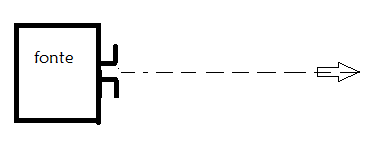
\includegraphics[scale=0.6]{fonte-eixo.png}
					\caption{Direção de propagação da onda EM }
					\label{fonte-eixo}
			\end{subfigure}
			\qquad
			\begin{subfigure}[b]{0.3\textwidth}
					\centering					
					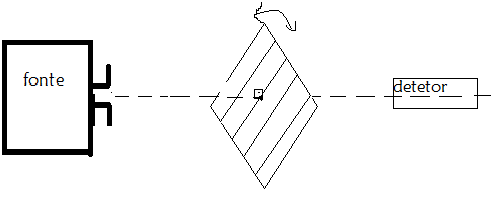
\includegraphics[scale=0.6]{grade-polarizadora.png}
					\caption{procedimento 3 }
					\label{grade-polarizadora}
			\end{subfigure}
			
			\begin{subfigure}[b]{0.3\textwidth}
					\centering					
					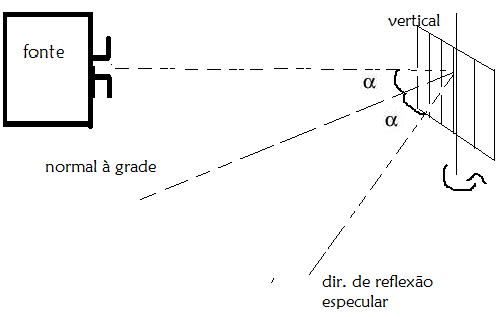
\includegraphics[scale=0.6]{grade-reflexao.png}
					\caption{procedimento 4}
					\label{grade-reflexão}
			\end{subfigure}

			\begin{subfigure}[b]{0.3\textwidth}
					\centering					
					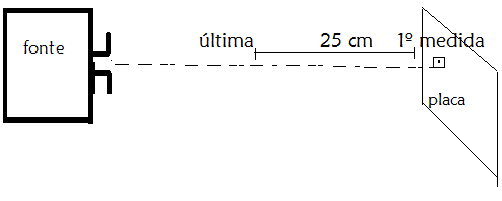
\includegraphics[scale=0.6]{placa.png}
					\caption{procedimento 5}
					\label{placa}
			\end{subfigure}
			
			
	\caption{Esquema das montagens}
	\end{figure}
\FloatBarrier

%@@@@@@@@@@@@@@@@@@@@@@@@@@@@@@@@@@@@@@@@@@@@@@@@@@@@@@@@@@@
%@@@@@@@@@@@@@@@@@@@       DADOS      @@@@@@@@@@@@@@@@@@@@@@
%@@@@@@@@@@@@@@@@@@@@@@@@@@@@@@@@@@@@@@@@@@@@@@@@@@@@@@@@@@@
\newpage
\section{Dados}

	\subsection{Observando $ \vec{E} $ e $ \vec{B} $}
	\paragraph{}	Para essa observação definimos os eixos como na figura \ref{eixos}. Nessa representação a direção de propagação da onda é ao longo do eixo \textbf{x} e a antena emissora esta na origem na direção do eixo y.  
		\begin{figure}[!htp]
 			 \centering
  			  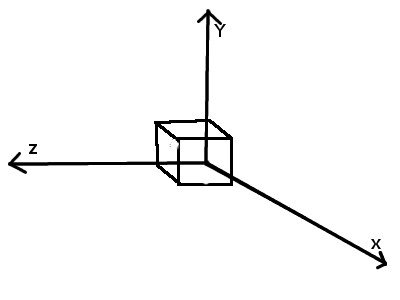
\includegraphics[scale = 0.5]{eixos.jpg}
  				\caption{Definindo os eixos}
  				\label{eixos}
		\end{figure}
		
	\paragraph{}Obtemos os resultados:
	\begin{itemize}
	

		\item Colocando a antena detectora de $ \vec{E} $ paralela a cada um dos eixos obtemos a tabela:

	\begin{table}[!htp]
		\centering	
		\begin{tabular}{|c|c|}\hline
		Eixo paralelo & Corrente $\pm 5 \mu A$  \\ \hline 
		x & 20 $\mu A$ \\ \hline
		y & 250 $\mu A$\\ \hline
		z & 0 $\mu A$\\ \hline	
		\end{tabular}
		\caption{Corrente em função da posição do detector $ \vec{E} $}
		\label{E-tab}
	\end{table}
	
	\item Colocando a espira do detector $ \vec{B} $ perpendicular a cada um dos eixos obtemos a tabela:
	\begin{table}[!htp]
		\centering	
		\begin{tabular}{|c|c|}\hline
		Eixo perpendicular & Corrente $\pm 0.5 \mu A$ \\ \hline 
		x & 0 $\mu A$ \\ \hline
		y & 0 $\mu A$\\ \hline
		z & 30 $\mu A$\\ \hline	
		\end{tabular}
		\caption{Corrente em função da posição do detector $ \vec{B} $}
		\label{B-tab}
	\end{table}


	\end{itemize}
	

\subsection{A grade polarizadora}
	\paragraph{}Na tabela a seguir orientamos a grade pelas suas barras. Dizemos que a grade esta à 0º quando suas barras estão paralelas ao eixo y e 90º quando paralelas ao eixo x.
	
	\begin{table}[!htp]
		\centering	
		\begin{tabular}{|c|c|}\hline
		Condição & Corrente $\pm 5 \mu A$  \\ \hline 
		sem grade & 150 $\mu A$ \\ \hline
		0º  & 0 $\mu A$\\ \hline
		45º & 45 $\mu A$\\ \hline	
		90º & 100 $\mu A$\\ \hline			
		\end{tabular}
		\caption{Corrente em função da orientação da grade metálica}
		\label{E-grad-tab}
	\end{table}

\subsection{Reflexão pela grade}

\paragraph{}Na tabela \ref{E-grad-refletida} anotamos a corrente medida pela detector em cada posição. 

	\begin{table}[!htp]
		\centering	
		\begin{tabular}{|l|c|}\hline
		Condição		 				& Corrente $\pm 5 \mu A$  \\ \hline 
		Onda que passa pela grade	 & 0$\mu A$ \\ \hline		
		Onda refletida na direção especular  & 160 $\mu A$ \\ \hline
		Sem grade   		& 200 $\mu A$\\ \hline
		
		\end{tabular}
		\caption{Onda refletida pela grade}
		\label{E-grad-refletida}	
	\end{table}
	

\subsection{O campo estacionário}
\paragraph{} A tabela \ref{tab-E-B-refletido} foi obtida medindo os campos $\vec{E}$ e $\vec{B}$ a partir da placa refletora. Os gráficos nas figuras \ref{graph-E} e \ref{graph-B} mostram os dados da tabela junto com a curva na fórmula \ref{formula-regressao} que melhor se adapta ao dados. A figura \ref{graph-B-E-extrapolado} mostra as duas curvas achadas por regressão para as amplitudes dos campos da onda estacionária. 

\FloatBarrier
\begin{flushleft}


\begin{table}[!htp]

		\begin{tabular}{|c|c|c|} \hline 
			\backslashbox{Dist.(cm) }{Campo  $ (\mu A)$}  & $ \vec{E} $ & $ \vec{B} $ \\ \hline
		 1.00 & 45.00 & - \\ \hline 
		 1.50 & 70.00 & - \\ \hline 
		 2.00 & 80.00 & - \\ \hline 
		 2.50 & 70.00 & - \\ \hline 
		 3.00 & 55.00 & 0.00 \\ \hline 
		 3.50 & 40.00 & 1.00 \\ \hline 
		 4.00 & 25.00 & 3.00 \\ \hline 
		 4.50 & 15.00 & 5.50 \\ \hline 
		 5.00 & 5.00 & 9.00 \\ \hline 
		 5.50 & 2.00 & 10.00 \\ \hline 
		 6.00 & 2.00 & 7.00 \\ \hline 
		 6.50 & 10.00 & 5.00 \\ \hline 
		 7.00 & 30.00 & 2.50 \\ \hline 
		 7.50 & 60.00 & 1.00 \\ \hline 
		 8.00 & 75.00 & 2.00 \\ \hline 
		 8.50 & 75.00 & 3.00 \\ \hline 
		 9.00 & 55.00 & 4.00 \\ \hline 
		 9.50 & 35.00 & 5.00 \\ \hline 
		 10.00 & 20.00 & 6.00 \\ \hline 
		 10.50 & 10.00 & 8.00 \\ \hline 
		\end{tabular}
	\begin{tabular}{|c|c|c|} \hline
	\backslashbox{Dist.(cm) }{Campo  $ (\mu A) $}  & $ \vec{E} $ & $ \vec{B} $ \\ \hline
		 11.00 & 3.00 & 10.00 \\ \hline 
		 11.50 & 3.00 & 11.00 \\ \hline 
		 12.00 & 10.00 & 9.00 \\ \hline 
		 12.50 & 25.00 & 6.00 \\ \hline 
		 13.00 & 55.00 & 5.00 \\ \hline 
		 13.50 & 75.00 & 3.00 \\ \hline 
		 14.00 & 80.00 & 2.00 \\ \hline 
		 14.50 & 75.00 & 1.00 \\ \hline 
		 15.00 & 60.00 & 2.00 \\ \hline 
		 15.50 & 50.00 & 2.00 \\ \hline 
		 16.00 & 35.00 & 4.00 \\ \hline 
		 16.50 & 15.00 & 7.00 \\ \hline 
		 17.00 & 5.00 & 9.00 \\ \hline 
		 17.50 & 5.00 & 10.00 \\ \hline 
		 18.00 & 10.00 & 8.00 \\ \hline 
		 18.50 & 40.00 & 7.00 \\ \hline 
		 19.00 & 60.00 & 5.00 \\ \hline 
		 19.50 & 75.00 & 3.00 \\ \hline 
		 20.00 & 80.00 & 2.00 \\ \hline 
		 20.50 & - & 2.00 \\ \hline 
		 21.00 & - & 3.00 \\ \hline 
		 21.00 & - & 3.00 \\ \hline 
	\end{tabular}	  
 	\caption{Intensidade de corrente medida pela distância } 
 	\label{tab-E-B-refletido}
 \end{table}
 \end{flushleft}

\FloatBarrier
			\begin{figure}[b]
					\centering
					% GNUPLOT: LaTeX picture with Postscript
\begingroup
  \makeatletter
  \providecommand\color[2][]{%
    \GenericError{(gnuplot) \space\space\space\@spaces}{%
      Package color not loaded in conjunction with
      terminal option `colourtext'%
    }{See the gnuplot documentation for explanation.%
    }{Either use 'blacktext' in gnuplot or load the package
      color.sty in LaTeX.}%
    \renewcommand\color[2][]{}%
  }%
  \providecommand\includegraphics[2][]{%
    \GenericError{(gnuplot) \space\space\space\@spaces}{%
      Package graphicx or graphics not loaded%
    }{See the gnuplot documentation for explanation.%
    }{The gnuplot epslatex terminal needs graphicx.sty or graphics.sty.}%
    \renewcommand\includegraphics[2][]{}%
  }%
  \providecommand\rotatebox[2]{#2}%
  \@ifundefined{ifGPcolor}{%
    \newif\ifGPcolor
    \GPcolorfalse
  }{}%
  \@ifundefined{ifGPblacktext}{%
    \newif\ifGPblacktext
    \GPblacktexttrue
  }{}%
  % define a \g@addto@macro without @ in the name:
  \let\gplgaddtomacro\g@addto@macro
  % define empty templates for all commands taking text:
  \gdef\gplbacktext{}%
  \gdef\gplfronttext{}%
  \makeatother
  \ifGPblacktext
    % no textcolor at all
    \def\colorrgb#1{}%
    \def\colorgray#1{}%
  \else
    % gray or color?
    \ifGPcolor
      \def\colorrgb#1{\color[rgb]{#1}}%
      \def\colorgray#1{\color[gray]{#1}}%
      \expandafter\def\csname LTw\endcsname{\color{white}}%
      \expandafter\def\csname LTb\endcsname{\color{black}}%
      \expandafter\def\csname LTa\endcsname{\color{black}}%
      \expandafter\def\csname LT0\endcsname{\color[rgb]{1,0,0}}%
      \expandafter\def\csname LT1\endcsname{\color[rgb]{0,1,0}}%
      \expandafter\def\csname LT2\endcsname{\color[rgb]{0,0,1}}%
      \expandafter\def\csname LT3\endcsname{\color[rgb]{1,0,1}}%
      \expandafter\def\csname LT4\endcsname{\color[rgb]{0,1,1}}%
      \expandafter\def\csname LT5\endcsname{\color[rgb]{1,1,0}}%
      \expandafter\def\csname LT6\endcsname{\color[rgb]{0,0,0}}%
      \expandafter\def\csname LT7\endcsname{\color[rgb]{1,0.3,0}}%
      \expandafter\def\csname LT8\endcsname{\color[rgb]{0.5,0.5,0.5}}%
    \else
      % gray
      \def\colorrgb#1{\color{black}}%
      \def\colorgray#1{\color[gray]{#1}}%
      \expandafter\def\csname LTw\endcsname{\color{white}}%
      \expandafter\def\csname LTb\endcsname{\color{black}}%
      \expandafter\def\csname LTa\endcsname{\color{black}}%
      \expandafter\def\csname LT0\endcsname{\color{black}}%
      \expandafter\def\csname LT1\endcsname{\color{black}}%
      \expandafter\def\csname LT2\endcsname{\color{black}}%
      \expandafter\def\csname LT3\endcsname{\color{black}}%
      \expandafter\def\csname LT4\endcsname{\color{black}}%
      \expandafter\def\csname LT5\endcsname{\color{black}}%
      \expandafter\def\csname LT6\endcsname{\color{black}}%
      \expandafter\def\csname LT7\endcsname{\color{black}}%
      \expandafter\def\csname LT8\endcsname{\color{black}}%
    \fi
  \fi
  \setlength{\unitlength}{0.0500bp}%
  \begin{picture}(7200.00,5040.00)%
    \gplgaddtomacro\gplbacktext{%
      \csname LTb\endcsname%
      \put(814,704){\makebox(0,0)[r]{\strut{}-10}}%
      \put(814,1072){\makebox(0,0)[r]{\strut{} 0}}%
      \put(814,1439){\makebox(0,0)[r]{\strut{} 10}}%
      \put(814,1807){\makebox(0,0)[r]{\strut{} 20}}%
      \put(814,2174){\makebox(0,0)[r]{\strut{} 30}}%
      \put(814,2542){\makebox(0,0)[r]{\strut{} 40}}%
      \put(814,2909){\makebox(0,0)[r]{\strut{} 50}}%
      \put(814,3277){\makebox(0,0)[r]{\strut{} 60}}%
      \put(814,3644){\makebox(0,0)[r]{\strut{} 70}}%
      \put(814,4012){\makebox(0,0)[r]{\strut{} 80}}%
      \put(814,4379){\makebox(0,0)[r]{\strut{} 90}}%
      \put(946,484){\makebox(0,0){\strut{} 0}}%
      \put(1532,484){\makebox(0,0){\strut{} 2}}%
      \put(2117,484){\makebox(0,0){\strut{} 4}}%
      \put(2703,484){\makebox(0,0){\strut{} 6}}%
      \put(3289,484){\makebox(0,0){\strut{} 8}}%
      \put(3875,484){\makebox(0,0){\strut{} 10}}%
      \put(4460,484){\makebox(0,0){\strut{} 12}}%
      \put(5046,484){\makebox(0,0){\strut{} 14}}%
      \put(5632,484){\makebox(0,0){\strut{} 16}}%
      \put(6217,484){\makebox(0,0){\strut{} 18}}%
      \put(6803,484){\makebox(0,0){\strut{} 20}}%
      \put(176,2541){\makebox(0,0){\strut{}$i(\mu A)$}}%
      \put(3874,154){\makebox(0,0){\strut{}$d(cm)$}}%
      \put(3874,4709){\makebox(0,0){\strut{}Onda estacionária campo $\vec{E}$ vs distância da placa refletora}}%
    }%
    \gplgaddtomacro\gplfronttext{%
      \csname LTb\endcsname%
      \put(5816,4206){\makebox(0,0)[r]{\strut{}$75.36 \sin^2(\frac{2\pi(x - 5.26)}{11.87})$}}%
      \csname LTb\endcsname%
      \put(5816,3986){\makebox(0,0)[r]{\strut{}dados}}%
    }%
    \gplbacktext
    \put(0,0){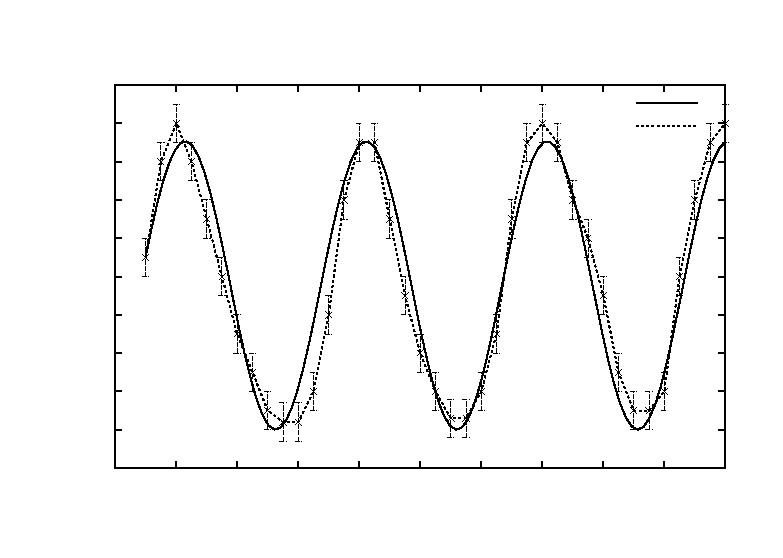
\includegraphics{./images/E-graph.eps}}%
    \gplfronttext
  \end{picture}%
\endgroup
  
					\caption{}
					\label{graph-E}
			\end{figure}

		
			\begin{figure}[b]		
					\centering
					% GNUPLOT: LaTeX picture with Postscript
\begingroup
  \makeatletter
  \providecommand\color[2][]{%
    \GenericError{(gnuplot) \space\space\space\@spaces}{%
      Package color not loaded in conjunction with
      terminal option `colourtext'%
    }{See the gnuplot documentation for explanation.%
    }{Either use 'blacktext' in gnuplot or load the package
      color.sty in LaTeX.}%
    \renewcommand\color[2][]{}%
  }%
  \providecommand\includegraphics[2][]{%
    \GenericError{(gnuplot) \space\space\space\@spaces}{%
      Package graphicx or graphics not loaded%
    }{See the gnuplot documentation for explanation.%
    }{The gnuplot epslatex terminal needs graphicx.sty or graphics.sty.}%
    \renewcommand\includegraphics[2][]{}%
  }%
  \providecommand\rotatebox[2]{#2}%
  \@ifundefined{ifGPcolor}{%
    \newif\ifGPcolor
    \GPcolorfalse
  }{}%
  \@ifundefined{ifGPblacktext}{%
    \newif\ifGPblacktext
    \GPblacktexttrue
  }{}%
  % define a \g@addto@macro without @ in the name:
  \let\gplgaddtomacro\g@addto@macro
  % define empty templates for all commands taking text:
  \gdef\gplbacktext{}%
  \gdef\gplfronttext{}%
  \makeatother
  \ifGPblacktext
    % no textcolor at all
    \def\colorrgb#1{}%
    \def\colorgray#1{}%
  \else
    % gray or color?
    \ifGPcolor
      \def\colorrgb#1{\color[rgb]{#1}}%
      \def\colorgray#1{\color[gray]{#1}}%
      \expandafter\def\csname LTw\endcsname{\color{white}}%
      \expandafter\def\csname LTb\endcsname{\color{black}}%
      \expandafter\def\csname LTa\endcsname{\color{black}}%
      \expandafter\def\csname LT0\endcsname{\color[rgb]{1,0,0}}%
      \expandafter\def\csname LT1\endcsname{\color[rgb]{0,1,0}}%
      \expandafter\def\csname LT2\endcsname{\color[rgb]{0,0,1}}%
      \expandafter\def\csname LT3\endcsname{\color[rgb]{1,0,1}}%
      \expandafter\def\csname LT4\endcsname{\color[rgb]{0,1,1}}%
      \expandafter\def\csname LT5\endcsname{\color[rgb]{1,1,0}}%
      \expandafter\def\csname LT6\endcsname{\color[rgb]{0,0,0}}%
      \expandafter\def\csname LT7\endcsname{\color[rgb]{1,0.3,0}}%
      \expandafter\def\csname LT8\endcsname{\color[rgb]{0.5,0.5,0.5}}%
    \else
      % gray
      \def\colorrgb#1{\color{black}}%
      \def\colorgray#1{\color[gray]{#1}}%
      \expandafter\def\csname LTw\endcsname{\color{white}}%
      \expandafter\def\csname LTb\endcsname{\color{black}}%
      \expandafter\def\csname LTa\endcsname{\color{black}}%
      \expandafter\def\csname LT0\endcsname{\color{black}}%
      \expandafter\def\csname LT1\endcsname{\color{black}}%
      \expandafter\def\csname LT2\endcsname{\color{black}}%
      \expandafter\def\csname LT3\endcsname{\color{black}}%
      \expandafter\def\csname LT4\endcsname{\color{black}}%
      \expandafter\def\csname LT5\endcsname{\color{black}}%
      \expandafter\def\csname LT6\endcsname{\color{black}}%
      \expandafter\def\csname LT7\endcsname{\color{black}}%
      \expandafter\def\csname LT8\endcsname{\color{black}}%
    \fi
  \fi
  \setlength{\unitlength}{0.0500bp}%
  \begin{picture}(7200.00,5040.00)%
    \gplgaddtomacro\gplbacktext{%
      \csname LTb\endcsname%
      \put(814,704){\makebox(0,0)[r]{\strut{}-2}}%
      \put(814,1229){\makebox(0,0)[r]{\strut{} 0}}%
      \put(814,1754){\makebox(0,0)[r]{\strut{} 2}}%
      \put(814,2279){\makebox(0,0)[r]{\strut{} 4}}%
      \put(814,2804){\makebox(0,0)[r]{\strut{} 6}}%
      \put(814,3329){\makebox(0,0)[r]{\strut{} 8}}%
      \put(814,3854){\makebox(0,0)[r]{\strut{} 10}}%
      \put(814,4379){\makebox(0,0)[r]{\strut{} 12}}%
      \put(946,484){\makebox(0,0){\strut{} 2}}%
      \put(1532,484){\makebox(0,0){\strut{} 4}}%
      \put(2117,484){\makebox(0,0){\strut{} 6}}%
      \put(2703,484){\makebox(0,0){\strut{} 8}}%
      \put(3289,484){\makebox(0,0){\strut{} 10}}%
      \put(3875,484){\makebox(0,0){\strut{} 12}}%
      \put(4460,484){\makebox(0,0){\strut{} 14}}%
      \put(5046,484){\makebox(0,0){\strut{} 16}}%
      \put(5632,484){\makebox(0,0){\strut{} 18}}%
      \put(6217,484){\makebox(0,0){\strut{} 20}}%
      \put(6803,484){\makebox(0,0){\strut{} 22}}%
      \put(176,2541){\makebox(0,0){\strut{}$i(\mu A)$}}%
      \put(3874,154){\makebox(0,0){\strut{}$d(cm)$}}%
      \put(3874,4709){\makebox(0,0){\strut{}Onda estacionária : campo $\vec{B}$ vs distância da placa refletora}}%
    }%
    \gplgaddtomacro\gplfronttext{%
      \csname LTb\endcsname%
      \put(5816,4206){\makebox(0,0)[r]{\strut{}$9.36 \sin^2(\frac{2\pi(x - 2.42)}{11.96})$}}%
      \csname LTb\endcsname%
      \put(5816,3986){\makebox(0,0)[r]{\strut{}dados}}%
    }%
    \gplbacktext
    \put(0,0){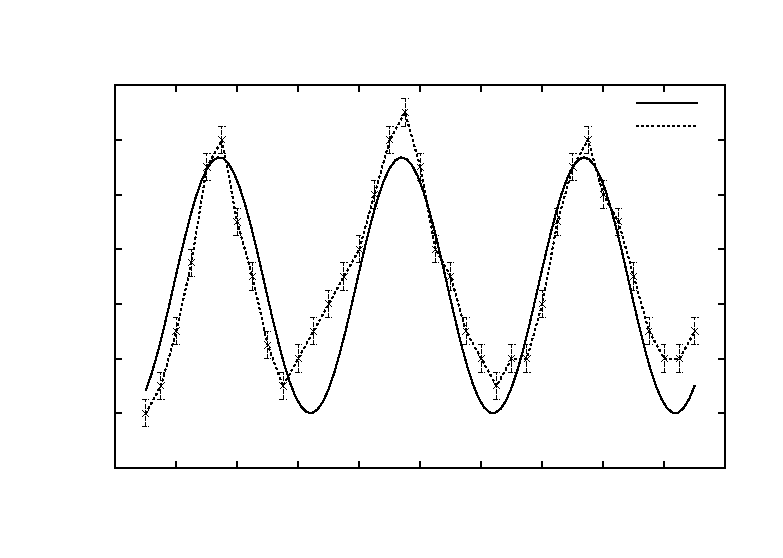
\includegraphics{./images/B-graph}}%
    \gplfronttext
  \end{picture}%
\endgroup
  
					\caption{}
					\label{graph-B}
			\end{figure}
			

\FloatBarrier

\FloatBarrier
			\begin{figure}[b]		
					\centering
					% GNUPLOT: LaTeX picture with Postscript
\begingroup
  \makeatletter
  \providecommand\color[2][]{%
    \GenericError{(gnuplot) \space\space\space\@spaces}{%
      Package color not loaded in conjunction with
      terminal option `colourtext'%
    }{See the gnuplot documentation for explanation.%
    }{Either use 'blacktext' in gnuplot or load the package
      color.sty in LaTeX.}%
    \renewcommand\color[2][]{}%
  }%
  \providecommand\includegraphics[2][]{%
    \GenericError{(gnuplot) \space\space\space\@spaces}{%
      Package graphicx or graphics not loaded%
    }{See the gnuplot documentation for explanation.%
    }{The gnuplot epslatex terminal needs graphicx.sty or graphics.sty.}%
    \renewcommand\includegraphics[2][]{}%
  }%
  \providecommand\rotatebox[2]{#2}%
  \@ifundefined{ifGPcolor}{%
    \newif\ifGPcolor
    \GPcolorfalse
  }{}%
  \@ifundefined{ifGPblacktext}{%
    \newif\ifGPblacktext
    \GPblacktexttrue
  }{}%
  % define a \g@addto@macro without @ in the name:
  \let\gplgaddtomacro\g@addto@macro
  % define empty templates for all commands taking text:
  \gdef\gplbacktext{}%
  \gdef\gplfronttext{}%
  \makeatother
  \ifGPblacktext
    % no textcolor at all
    \def\colorrgb#1{}%
    \def\colorgray#1{}%
  \else
    % gray or color?
    \ifGPcolor
      \def\colorrgb#1{\color[rgb]{#1}}%
      \def\colorgray#1{\color[gray]{#1}}%
      \expandafter\def\csname LTw\endcsname{\color{white}}%
      \expandafter\def\csname LTb\endcsname{\color{black}}%
      \expandafter\def\csname LTa\endcsname{\color{black}}%
      \expandafter\def\csname LT0\endcsname{\color[rgb]{1,0,0}}%
      \expandafter\def\csname LT1\endcsname{\color[rgb]{0,1,0}}%
      \expandafter\def\csname LT2\endcsname{\color[rgb]{0,0,1}}%
      \expandafter\def\csname LT3\endcsname{\color[rgb]{1,0,1}}%
      \expandafter\def\csname LT4\endcsname{\color[rgb]{0,1,1}}%
      \expandafter\def\csname LT5\endcsname{\color[rgb]{1,1,0}}%
      \expandafter\def\csname LT6\endcsname{\color[rgb]{0,0,0}}%
      \expandafter\def\csname LT7\endcsname{\color[rgb]{1,0.3,0}}%
      \expandafter\def\csname LT8\endcsname{\color[rgb]{0.5,0.5,0.5}}%
    \else
      % gray
      \def\colorrgb#1{\color{black}}%
      \def\colorgray#1{\color[gray]{#1}}%
      \expandafter\def\csname LTw\endcsname{\color{white}}%
      \expandafter\def\csname LTb\endcsname{\color{black}}%
      \expandafter\def\csname LTa\endcsname{\color{black}}%
      \expandafter\def\csname LT0\endcsname{\color{black}}%
      \expandafter\def\csname LT1\endcsname{\color{black}}%
      \expandafter\def\csname LT2\endcsname{\color{black}}%
      \expandafter\def\csname LT3\endcsname{\color{black}}%
      \expandafter\def\csname LT4\endcsname{\color{black}}%
      \expandafter\def\csname LT5\endcsname{\color{black}}%
      \expandafter\def\csname LT6\endcsname{\color{black}}%
      \expandafter\def\csname LT7\endcsname{\color{black}}%
      \expandafter\def\csname LT8\endcsname{\color{black}}%
    \fi
  \fi
  \setlength{\unitlength}{0.0500bp}%
  \begin{picture}(7200.00,5040.00)%
    \gplgaddtomacro\gplbacktext{%
      \csname LTb\endcsname%
      \put(814,704){\makebox(0,0)[r]{\strut{} 0}}%
      \put(814,1156){\makebox(0,0)[r]{\strut{} 10}}%
      \put(814,1609){\makebox(0,0)[r]{\strut{} 20}}%
      \put(814,2061){\makebox(0,0)[r]{\strut{} 30}}%
      \put(814,2513){\makebox(0,0)[r]{\strut{} 40}}%
      \put(814,2966){\makebox(0,0)[r]{\strut{} 50}}%
      \put(814,3418){\makebox(0,0)[r]{\strut{} 60}}%
      \put(814,3870){\makebox(0,0)[r]{\strut{} 70}}%
      \put(814,4323){\makebox(0,0)[r]{\strut{} 80}}%
      \put(814,4775){\makebox(0,0)[r]{\strut{} 90}}%
      \put(946,484){\makebox(0,0){\strut{} 0}}%
      \put(2410,484){\makebox(0,0){\strut{} 5}}%
      \put(3875,484){\makebox(0,0){\strut{} 10}}%
      \put(5339,484){\makebox(0,0){\strut{} 15}}%
      \put(6803,484){\makebox(0,0){\strut{} 20}}%
      \put(176,2739){\makebox(0,0){\strut{}$i(\mu A)$}}%
      \put(3874,154){\makebox(0,0){\strut{}$d(cm)$}}%
    }%
    \gplgaddtomacro\gplfronttext{%
      \csname LTb\endcsname%
      \put(5816,4602){\makebox(0,0)[r]{\strut{}E(x)}}%
      \csname LTb\endcsname%
      \put(5816,4382){\makebox(0,0)[r]{\strut{}B(x)}}%
    }%
    \gplbacktext
    \put(0,0){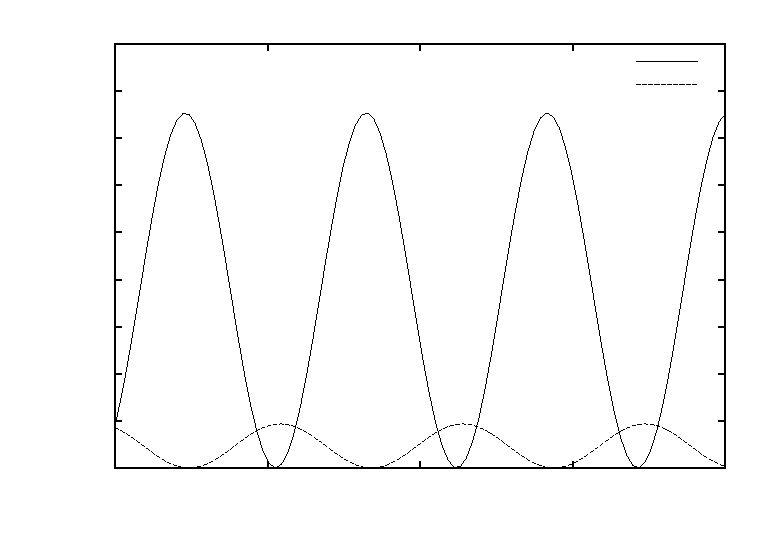
\includegraphics{B-E-regres}}%
    \gplfronttext
  \end{picture}%
\endgroup
  
					\caption{Curvas para $\vec{E}$ e $\vec{B}$ extrapoladas }
					\label{graph-B-E-extrapolado}
			\end{figure}
\FloatBarrier

%@@@@@@@@@@@@@@@@@@@@@@@@@@@@@@@@@@@@@@@@@@@@@@@@@@@@@@@@@@@
%@@@@@@@@@@@@@@       Análise         @@@@@@@@@@@@@@@@@@@@@@
%@@@@@@@@@@@@@@@@@@@@@@@@@@@@@@@@@@@@@@@@@@@@@@@@@@@@@@@@@@@

\section{Análise de Dados}
	\subsection{Observando $\vec{E}$ e $\vec{B}$}	
	
		\paragraph{}Observamos pela análise da tabela \ref{E-tab} que o sensor de campo elétrico produz corrente se as antenas estiverem paralelas ao eixo y, como vimos na introdução esse deve ser o eixo de oscilação do campo elétrico gerado pela antena. Observando a tabela \ref{B-tab} vemos que a corrente é máxima quando a espira está perpendicular ao eixo z. O eixo z é então o eixo no qual o campo magnético oscila. Notamos que os eixos nos quais os campos oscilam (y e z) são perpendiculares entre si e perpendiculares com o eixo x de propagação da onda.
		
	\subsection{A grade polarizadora}
		\paragraph{}	Colocamos uma grade com as suas barras de forma paralela à oscilação do campo elétrico a frente do detetor. O esperado caso fosse uma onda numa corda, por exemplo, era que a mesma passasse normalmente pela fissura entre as grades. Entretanto, nessa situação não vemos nenhuma corrente no amperímetro.Ou seja, a onda não passa pela grade. Isso acontece porque diferente da onda numa corda, a onda elétrica interage com a grade. 
	\paragraph{} Os elétrons na grade estão livres para se movimentarem.Quando o campo elétrico passa por eles a energia sendo transportada pela onda é transformada em energia cinética pelas cargas livres. Esse processo 'mata' a onda EM.
	
	\paragraph{} Ao colocarmos a grade perpendicular ao campo pudemos medir a onda elétrica, isso porque as barras não mais teriam o sentido de oscilação da onda, fazendo com que os elétrons não se movessem com tanta liberdade quanto estavam se movendo no caso anterior. 
	
	\paragraph{} É valido ressaltar que mesmo com a grade perpendicular parte da energia foi perdida nela, pois ao medirmos sem a grade e com a grade, notávamos uma diferença de aproximadamente 30\% na medida da corrente. Isso talvez tenha se dado devido a espessura das grades não serem desprezíveis e por haver barras paralelas na lateral da grade que poderiam reter parte da energia.
	
	\subsection{Reflexão pela grade}
	
	\paragraph{} Como podemos ver na tabela \ref{E-grad-refletida}, a parte refletida foi maior que a dissipada, o que era de se esperar já que a reflexão é na verdade uma “nova” onda gerada pelo movimento dos elétrons que foi gerado pela onda anterior, acredita-se que o restante foi perdido em forma de calor por efeito joule, já que não havia resquícios de onda atrás das grades mesmo neste ângulo.
	
	\paragraph{O campo estacionário}
	
	\paragraph{}Nesta parte do experimento onde elas se comportam de forma estacionária, pudemos observar no gráfico \ref{graph-B-E-extrapolado} que elas estão com seus máximos e mínimos defasados por $\frac{\lambda}{2}$, ou seja, quando o campo elétrico é máximo o magnético é mínimo e vise versa. Isso concorda com o esperado em teoria pelas fórmulas \ref{formula-estacionaria}.
	
	\paragraph{} Como visto nos gráficos \ref{graph-E} e \ref{graph-B} e comparando com a fórmula \ref{formula-regressao} obtemos que o comprimento de onda $\lambda$ para a onda em estudo é:
	
	\begin{displaymath}
		\lambda = 11.9 \quad cm 
	\end{displaymath}
	
	\paragraph{}Podemos então usar a relação $c = \lambda f$ e supor a velocidade da luz como igual a do vácuo para obter:
	\begin{displaymath}
		f = \frac{c}{\lambda} = \frac{299792458 m/s}{0.119 m} = 2.5193 \quad GHz 
	\end{displaymath}
	
	\paragraph{}Podemos usar as fórmulas novamente para obter as intensidades dos campos na origem.
	\begin{displaymath}	
		E(0) = 75.36 \sin^2(\frac{2\pi(0 - 5.26)}{11.87}) =  9.21 
	\end{displaymath}
	\begin{displaymath}	
		B(0) = 9.36 \sin^2(\frac{2\pi(x - 2.42)}{11.96}) =   8.54	
	\end{displaymath}
	
	\paragraph{} Era esperado que $E(0)$ fosse 0 na origem e que o campo 	$B(0)$ estivesse em 9.36, seu máximo. Os valores estão dentro do esperado devido aos erros associados. Qualitativamente, podemos dizer que $E(0)$ esta próximo de seu mínimo e $B(0)$ próximo de seu máximo.  
	
	\paragraph{}Vamos agora calcular o vetor de Poyting. Esse vetor mede a intensidade da radiação eletromagnética e indica sua direção de propagação. Ele é dado por:
		
	\begin{equation}
		\vec{S} = \frac{1}{\mu_0} \vec{E} \times \vec{B}
	\end{equation}
	
	\paragraph{} Como $\vec{S}$ varia muito rapidamente em geral analisamos o sue valor médio ao longo de um período. Já vimos na introdução que para uma onda estacionária os vetores $\vec{E}$ e $\vec{B}$ são dados pelas fórmulas \ref{formula-estacionaria}.Supondo o campo $\vec{E}$ na direção $\vec{y}$ e $\vec{B}$ em $\vec{z}$ seu produto será dado por:
	
	\begin{equation}
		\vec{S} = \frac{1}{\mu_0} (-4 E_{max}B_{max}\cos (kx) \sin (kx) \cos (wt) \sin (wt), 0, 0)
	\end{equation}
	
	\paragraph{}E sua média será dado por:
	
	\begin{displaymath}
		\overline{S} = \frac{\frac{-4 E_{max}B_{max}\cos (wt) \sin (wt)}{\mu_0} \int _0 ^{\lambda} \cos (kx) \sin (kx) dx}{\lambda}
	\end{displaymath}
	
	\paragraph{}Lembramos que $k = \frac{2 \pi}{\lambda}$ para obter:
	\begin{displaymath}
		\overline{S} = \frac{A(t) \int _0 ^{\lambda} \frac{\sin (\frac{2 \pi}{\lambda}x)}{2} dx}{\lambda} = \frac{A(t)  [\frac{\cos (\frac{2 \pi}{\lambda}x)}{4\pi / \lambda} ]_0^{^{\lambda}}}{\lambda} = 0	
	\end{displaymath}
	
	\paragraph{} Portanto, na média não há transferência de energia de um ponto para o outro do espaço entre a fonte e a placa refletora.
	
	

	
	


	
	
	
	

%@@@@@@@@@@@@@@@@@@@@@@@@@@@@@@@@@@@@@@@@@@@@@@@@@@@@@@@@@@@
%@@@@@@@@@@@@@@       CONCLUSAO       @@@@@@@@@@@@@@@@@@@@@@
%@@@@@@@@@@@@@@@@@@@@@@@@@@@@@@@@@@@@@@@@@@@@@@@@@@@@@@@@@@@
\section{Conclusão}

\paragraph{} Durante o experimento foi possível verificar a ortogonalidade dos campos elétrico e magnético e da direção de propagação da onda eletromagnética. Observou-se ainda a propriedade polarizadora de uma grade feita de material condutor e como esta reflete a maior parte da radiação recebida. Finalmente, observamos e analisamos a formação de uma onda eletromagnética estacionária. Portanto, considerando o erro intrínseco a toda medida, os experimentos foram bem sucedidos.    


%@@@@@@@@@@@@@@@@@@@@@@@@@@@@@@@@@@@@@@@@@@@@@@@@@@@@@@@@@@@
%@@@@@@@@@@@@@@       REFERÊNCIAS     @@@@@@@@@@@@@@@@@@@@@@
%@@@@@@@@@@@@@@@@@@@@@@@@@@@@@@@@@@@@@@@@@@@@@@@@@@@@@@@@@@@
\begin{thebibliography}{9}
	 \bibitem{fis2}
  		HALLIDAY, D.; RESNICK, R. ; WALKER.
  		\emph{Fundamentos de Física} volume 2 : Gravitação, Ondas e Termodinâmica.
 		 8ª ed.
 		 Rio de Janeiro : LTC, 2009.
    
	 \bibitem{fis3}
  		HALLIDAY, D.; RESNICK, R. ; WALKER.
  		\emph{Fundamentos de Física} volume 3 : Eletromagnetismo.
 		 8ª ed.
 		 Rio de Janeiro : LTC, 2009.

\end{thebibliography}



\end{document}
